% Options for packages loaded elsewhere
\PassOptionsToPackage{unicode}{hyperref}
\PassOptionsToPackage{hyphens}{url}
%
\documentclass[
  ignorenonframetext,
]{beamer}
\usepackage{pgfpages}
\setbeamertemplate{caption}[numbered]
\setbeamertemplate{caption label separator}{: }
\setbeamercolor{caption name}{fg=normal text.fg}
\beamertemplatenavigationsymbolsempty
% Prevent slide breaks in the middle of a paragraph
\widowpenalties 1 10000
\raggedbottom
\setbeamertemplate{part page}{
  \centering
  \begin{beamercolorbox}[sep=16pt,center]{part title}
    \usebeamerfont{part title}\insertpart\par
  \end{beamercolorbox}
}
\setbeamertemplate{section page}{
  \centering
  \begin{beamercolorbox}[sep=12pt,center]{part title}
    \usebeamerfont{section title}\insertsection\par
  \end{beamercolorbox}
}
\setbeamertemplate{subsection page}{
  \centering
  \begin{beamercolorbox}[sep=8pt,center]{part title}
    \usebeamerfont{subsection title}\insertsubsection\par
  \end{beamercolorbox}
}
\AtBeginPart{
  \frame{\partpage}
}
\AtBeginSection{
  \ifbibliography
  \else
    \frame{\sectionpage}
  \fi
}
\AtBeginSubsection{
  \frame{\subsectionpage}
}

\usepackage{amsmath,amssymb}
\usepackage{iftex}
\ifPDFTeX
  \usepackage[T1]{fontenc}
  \usepackage[utf8]{inputenc}
  \usepackage{textcomp} % provide euro and other symbols
\else % if luatex or xetex
  \usepackage{unicode-math}
  \defaultfontfeatures{Scale=MatchLowercase}
  \defaultfontfeatures[\rmfamily]{Ligatures=TeX,Scale=1}
\fi
\usepackage{lmodern}
\ifPDFTeX\else  
    % xetex/luatex font selection
\fi
% Use upquote if available, for straight quotes in verbatim environments
\IfFileExists{upquote.sty}{\usepackage{upquote}}{}
\IfFileExists{microtype.sty}{% use microtype if available
  \usepackage[]{microtype}
  \UseMicrotypeSet[protrusion]{basicmath} % disable protrusion for tt fonts
}{}
\makeatletter
\@ifundefined{KOMAClassName}{% if non-KOMA class
  \IfFileExists{parskip.sty}{%
    \usepackage{parskip}
  }{% else
    \setlength{\parindent}{0pt}
    \setlength{\parskip}{6pt plus 2pt minus 1pt}}
}{% if KOMA class
  \KOMAoptions{parskip=half}}
\makeatother
\usepackage{xcolor}
\newif\ifbibliography
\setlength{\emergencystretch}{3em} % prevent overfull lines
\setcounter{secnumdepth}{-\maxdimen} % remove section numbering


\providecommand{\tightlist}{%
  \setlength{\itemsep}{0pt}\setlength{\parskip}{0pt}}\usepackage{longtable,booktabs,array}
\usepackage{calc} % for calculating minipage widths
\usepackage{caption}
% Make caption package work with longtable
\makeatletter
\def\fnum@table{\tablename~\thetable}
\makeatother
\usepackage{graphicx}
\makeatletter
\def\maxwidth{\ifdim\Gin@nat@width>\linewidth\linewidth\else\Gin@nat@width\fi}
\def\maxheight{\ifdim\Gin@nat@height>\textheight\textheight\else\Gin@nat@height\fi}
\makeatother
% Scale images if necessary, so that they will not overflow the page
% margins by default, and it is still possible to overwrite the defaults
% using explicit options in \includegraphics[width, height, ...]{}
\setkeys{Gin}{width=\maxwidth,height=\maxheight,keepaspectratio}
% Set default figure placement to htbp
\makeatletter
\def\fps@figure{htbp}
\makeatother
% definitions for citeproc citations
\NewDocumentCommand\citeproctext{}{}
\NewDocumentCommand\citeproc{mm}{%
  \begingroup\def\citeproctext{#2}\cite{#1}\endgroup}
\makeatletter
 % allow citations to break across lines
 \let\@cite@ofmt\@firstofone
 % avoid brackets around text for \cite:
 \def\@biblabel#1{}
 \def\@cite#1#2{{#1\if@tempswa , #2\fi}}
\makeatother
\newlength{\cslhangindent}
\setlength{\cslhangindent}{1.5em}
\newlength{\csllabelwidth}
\setlength{\csllabelwidth}{3em}
\newenvironment{CSLReferences}[2] % #1 hanging-indent, #2 entry-spacing
 {\begin{list}{}{%
  \setlength{\itemindent}{0pt}
  \setlength{\leftmargin}{0pt}
  \setlength{\parsep}{0pt}
  % turn on hanging indent if param 1 is 1
  \ifodd #1
   \setlength{\leftmargin}{\cslhangindent}
   \setlength{\itemindent}{-1\cslhangindent}
  \fi
  % set entry spacing
  \setlength{\itemsep}{#2\baselineskip}}}
 {\end{list}}
\usepackage{calc}
\newcommand{\CSLBlock}[1]{\hfill\break\parbox[t]{\linewidth}{\strut\ignorespaces#1\strut}}
\newcommand{\CSLLeftMargin}[1]{\parbox[t]{\csllabelwidth}{\strut#1\strut}}
\newcommand{\CSLRightInline}[1]{\parbox[t]{\linewidth - \csllabelwidth}{\strut#1\strut}}
\newcommand{\CSLIndent}[1]{\hspace{\cslhangindent}#1}

\makeatletter
\@ifpackageloaded{caption}{}{\usepackage{caption}}
\AtBeginDocument{%
\ifdefined\contentsname
  \renewcommand*\contentsname{Table of contents}
\else
  \newcommand\contentsname{Table of contents}
\fi
\ifdefined\listfigurename
  \renewcommand*\listfigurename{List of Figures}
\else
  \newcommand\listfigurename{List of Figures}
\fi
\ifdefined\listtablename
  \renewcommand*\listtablename{List of Tables}
\else
  \newcommand\listtablename{List of Tables}
\fi
\ifdefined\figurename
  \renewcommand*\figurename{Figure}
\else
  \newcommand\figurename{Figure}
\fi
\ifdefined\tablename
  \renewcommand*\tablename{Table}
\else
  \newcommand\tablename{Table}
\fi
}
\@ifpackageloaded{float}{}{\usepackage{float}}
\floatstyle{ruled}
\@ifundefined{c@chapter}{\newfloat{codelisting}{h}{lop}}{\newfloat{codelisting}{h}{lop}[chapter]}
\floatname{codelisting}{Listing}
\newcommand*\listoflistings{\listof{codelisting}{List of Listings}}
\makeatother
\makeatletter
\makeatother
\makeatletter
\@ifpackageloaded{caption}{}{\usepackage{caption}}
\@ifpackageloaded{subcaption}{}{\usepackage{subcaption}}
\makeatother
\ifLuaTeX
  \usepackage{selnolig}  % disable illegal ligatures
\fi
\usepackage{bookmark}

\IfFileExists{xurl.sty}{\usepackage{xurl}}{} % add URL line breaks if available
\urlstyle{same} % disable monospaced font for URLs
\hypersetup{
  pdftitle={MODELAGEM E PREVISÃO DO NÚMERO DE CASOS DE INTERNAÇÃO POR DOENÇAS DO APARELHO RESPIRATÓRIO NA CIDADE DE SÃO PAULO VIA LSTM},
  hidelinks,
  pdfcreator={LaTeX via pandoc}}

\title{MODELAGEM E PREVISÃO DO NÚMERO DE CASOS DE INTERNAÇÃO POR DOENÇAS
DO APARELHO RESPIRATÓRIO NA CIDADE DE SÃO PAULO VIA LSTM}
\author{}
\date{}

\begin{document}
\frame{\titlepage}

\begin{frame}{Introdução}
\phantomsection\label{introduuxe7uxe3o}
\begin{itemize}
\tightlist
\item
  Compreende-se que há uma estreita relação entre fatores climáticos e a
  saúde humana, especialmente no que se refere ao sistema respiratório.
\item
  Condições climáticas adversas podem aumentar a ocorrência de
  internações hospitalares e, em casos mais graves, levar a óbitos
  (Arbex 2012).
\end{itemize}
\end{frame}

\begin{frame}{Introdução}
\phantomsection\label{introduuxe7uxe3o-1}
\begin{itemize}
\tightlist
\item
  Na saúde pública, prever o número de internações esperadas em um
  determinado período é essencial para criação de políticas públicas e
  previsão de cenários de maior exigência dos serviços de sáudes para
  atender pacientes com problemas respiratórios.
\item
  Neste trabalho, fizemos um modelo capaz de prever o número de
  internações, utilizando uma classe de redes neurais apropriada para
  séries temporais, isto é, o LSTM.
\item
  O estudo concentra-se na modelagem e previsão do número de internações
  por doenças do sistema respiratório na cidade de São Paulo entre os
  anos de 2018 e 2019.
\end{itemize}
\end{frame}

\section{Materiais e Métodos}\label{materiais-e-muxe9todos}

\begin{frame}{Memória Longa de Curto Prazo (LSTM)}
\phantomsection\label{memuxf3ria-longa-de-curto-prazo-lstm}
\begin{itemize}
\tightlist
\item
  O LSTM é um tipo de rede neural da família de Redes Neurais
  Recorrentes (RNNs) que funcionam como uma espécie de diversos
  ``mensageiros'' que processam os dados que receberam, e transmitem
  isso para outros mensageiros.
\item
  Isso cria uma espécie de memória que é compartilhada entre eles e pode
  fornecer bons resultados como saídas.
\end{itemize}
\end{frame}

\begin{frame}{Memória Longa de Curto Prazo (LSTM)}
\phantomsection\label{memuxf3ria-longa-de-curto-prazo-lstm-1}
\begin{itemize}
\tightlist
\item
  Devido a ineficiência das RNNs tradicionais não conseguirem manter as
  memórias por longos prazos surgiu o LSTM para superar esse problema
  (Bengio 1994).
\item
  Diferentemente de redes neurais recorrentes padrões, ele tem uma
  estrutura mais complexa.
\end{itemize}
\end{frame}

\begin{frame}{Memória Longa de Curto Prazo (LSTM)}
\phantomsection\label{memuxf3ria-longa-de-curto-prazo-lstm-2}
\begin{figure}[H]

{\centering 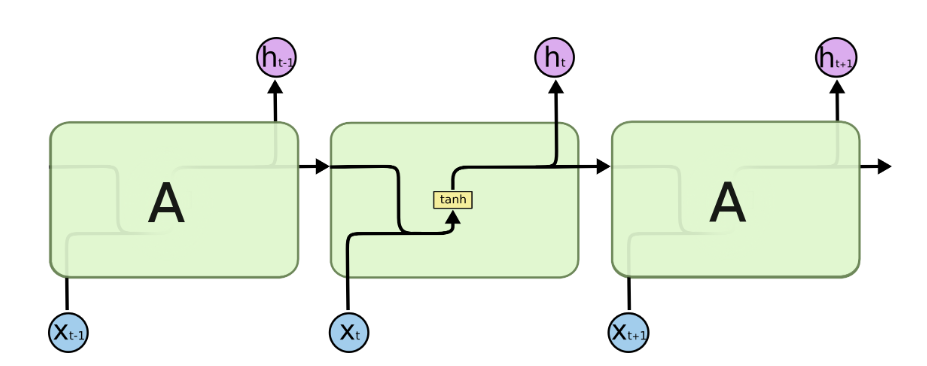
\includegraphics[width=3.09in,height=\textheight]{RNN_padrao.png}

}

\caption{RNN Padrão. Fonte:
https://colah.github.io/posts/2015-08-Understanding-LSTMs/}

\end{figure}%
\end{frame}

\begin{frame}{Memória Longa de Curto Prazo (LSTM)}
\phantomsection\label{memuxf3ria-longa-de-curto-prazo-lstm-3}
\begin{figure}[H]

{\centering 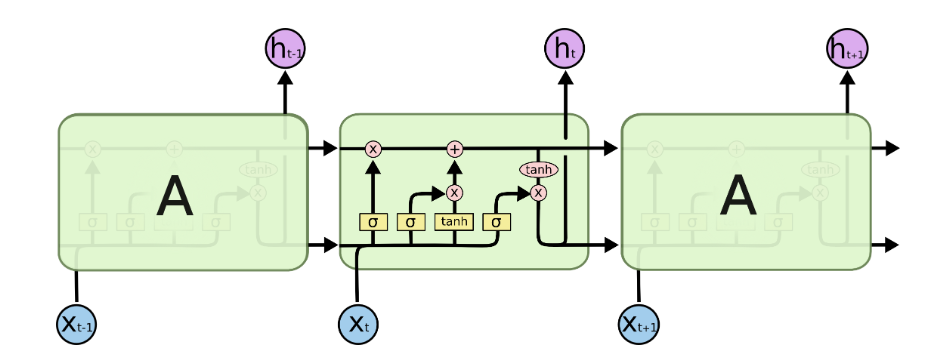
\includegraphics[width=3.11in,height=\textheight]{estrutura_lstm.png}

}

\caption{Fonte:
https://colah.github.io/posts/2015-08-Understanding-LSTMs/}

\end{figure}%
\end{frame}

\begin{frame}{Memória Longa de Curto Prazo (LSTM)}
\phantomsection\label{memuxf3ria-longa-de-curto-prazo-lstm-4}
\begin{figure}[H]

{\centering 
\includegraphics[width=3.13in,height=\textheight]{interconexao_info.png}

}

\caption{Fonte:
https://colah.github.io/posts/2015-08-Understanding-LSTMs/}

\end{figure}%
\end{frame}

\begin{frame}{Memória Longa de Curto Prazo (LSTM)}
\phantomsection\label{memuxf3ria-longa-de-curto-prazo-lstm-5}
\begin{figure}[H]

{\centering 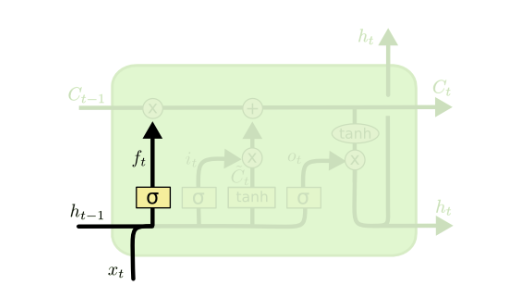
\includegraphics[width=1.69in,height=\textheight]{primeira_funcao.png}

}

\caption{Fonte:
https://colah.github.io/posts/2015-08-Understanding-LSTMs/}

\end{figure}%
\end{frame}

\begin{frame}{Memória Longa de Curto Prazo (LSTM)}
\phantomsection\label{memuxf3ria-longa-de-curto-prazo-lstm-6}
\begin{figure}[H]

{\centering 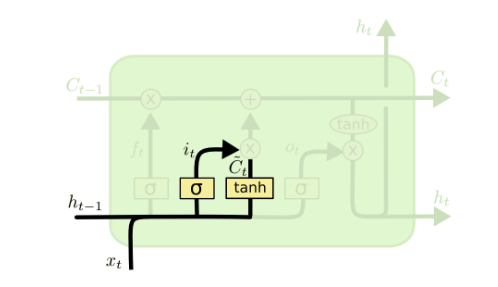
\includegraphics[width=1.66in,height=\textheight]{segunda_funcao.png}

}

\caption{Fonte:
https://colah.github.io/posts/2015-08-Understanding-LSTMs/}

\end{figure}%
\end{frame}

\begin{frame}{Memória Longa de Curto Prazo (LSTM)}
\phantomsection\label{memuxf3ria-longa-de-curto-prazo-lstm-7}
\begin{figure}[H]

{\centering 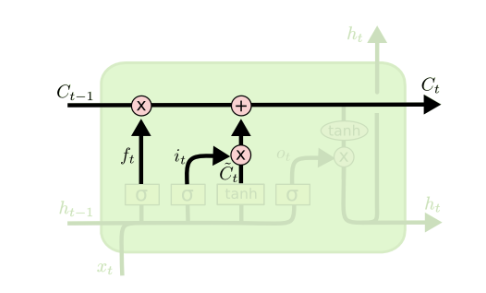
\includegraphics[width=1.62in,height=\textheight]{segunda_funcao_saida.png}

}

\caption{Fonte:
https://colah.github.io/posts/2015-08-Understanding-LSTMs/}

\end{figure}%
\end{frame}

\begin{frame}{Memória Longa de Curto Prazo (LSTM)}
\phantomsection\label{memuxf3ria-longa-de-curto-prazo-lstm-8}
\begin{figure}[H]

{\centering 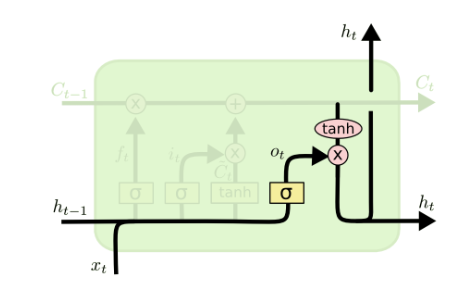
\includegraphics[width=1.57in,height=\textheight]{saida_final.png}

}

\caption{Fonte:
https://colah.github.io/posts/2015-08-Understanding-LSTMs/}

\end{figure}%
\end{frame}

\begin{frame}{Base de Dadoss}
\phantomsection\label{base-de-dadoss}
\begin{itemize}
\tightlist
\item
  Variável Alvo: Número de Internações por Doenças do Aparelho
  Respiratório;
\item
  Covariáveis: Material Particulado Fino, Temperatura Média e Umidade
  Relativa do Ar Média;
\item
  Fontes: DATASUS e Sistema Integrado de Serviços Ambientais (SISAM);
\item
  Frequência: Diária;
\item
  Período: 01/01/2018 a 30/11/2019.
\item
  Local: São Paulo - SP
\end{itemize}
\end{frame}

\section{Resultados}\label{resultados}

\begin{frame}{Análise Descritiva}
\phantomsection\label{anuxe1lise-descritiva}
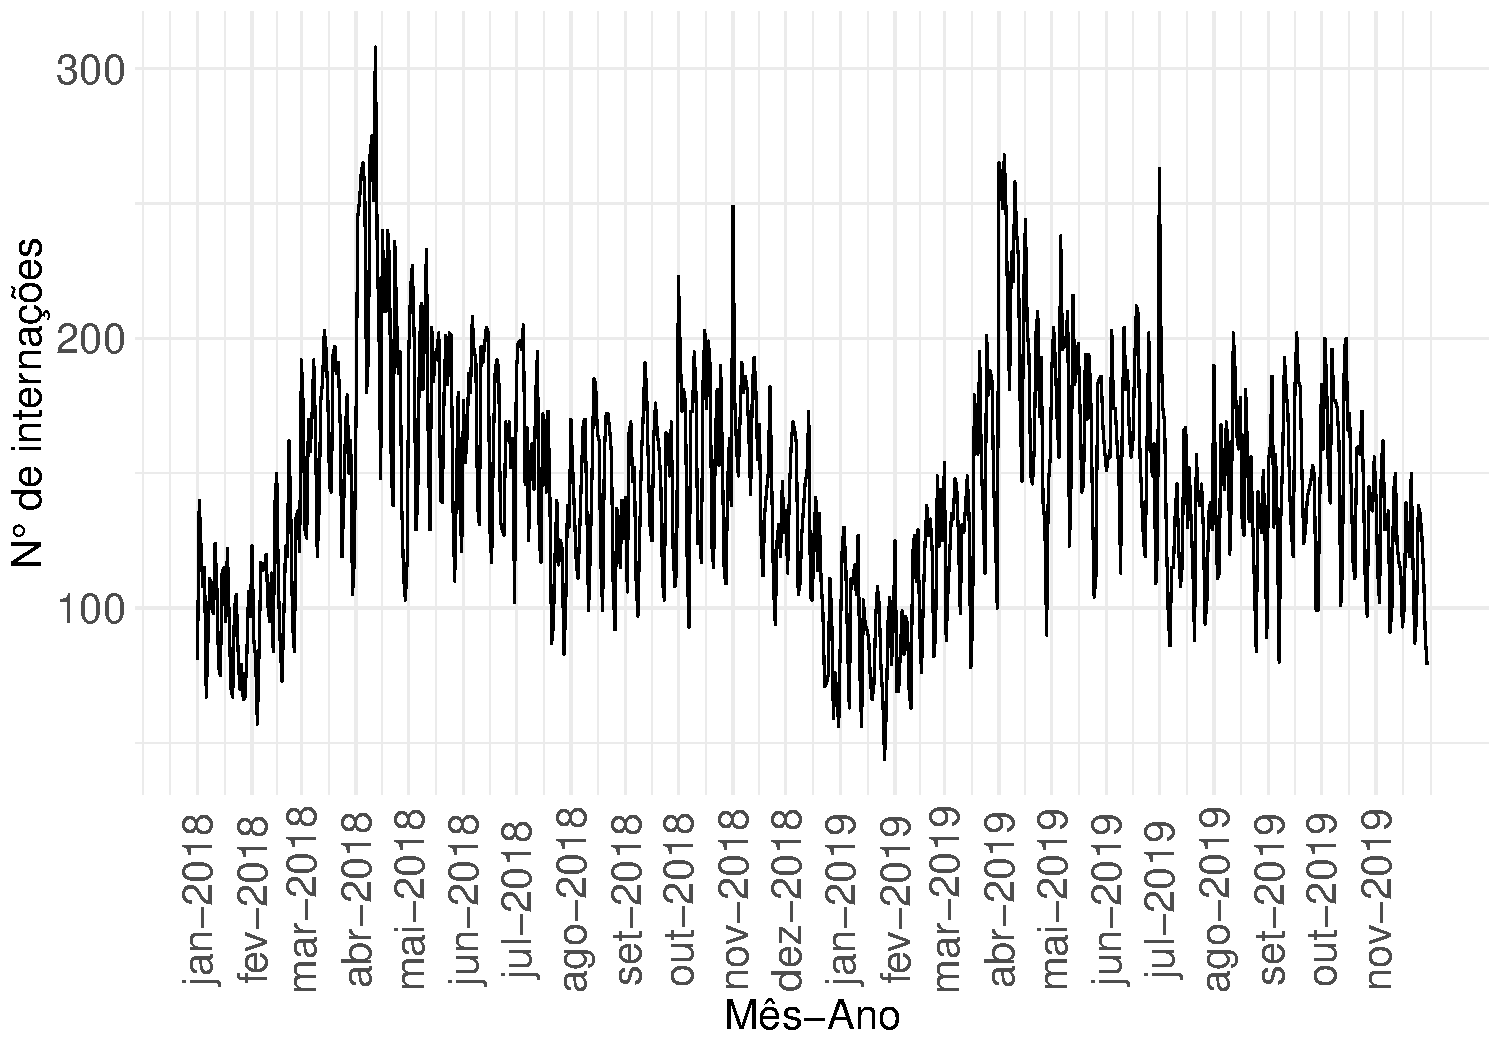
\includegraphics[width=1\textwidth,height=\textheight]{apresentacao_files/figure-beamer/unnamed-chunk-8-1.pdf}
\end{frame}

\begin{frame}{Análise Descritiva}
\phantomsection\label{anuxe1lise-descritiva-1}
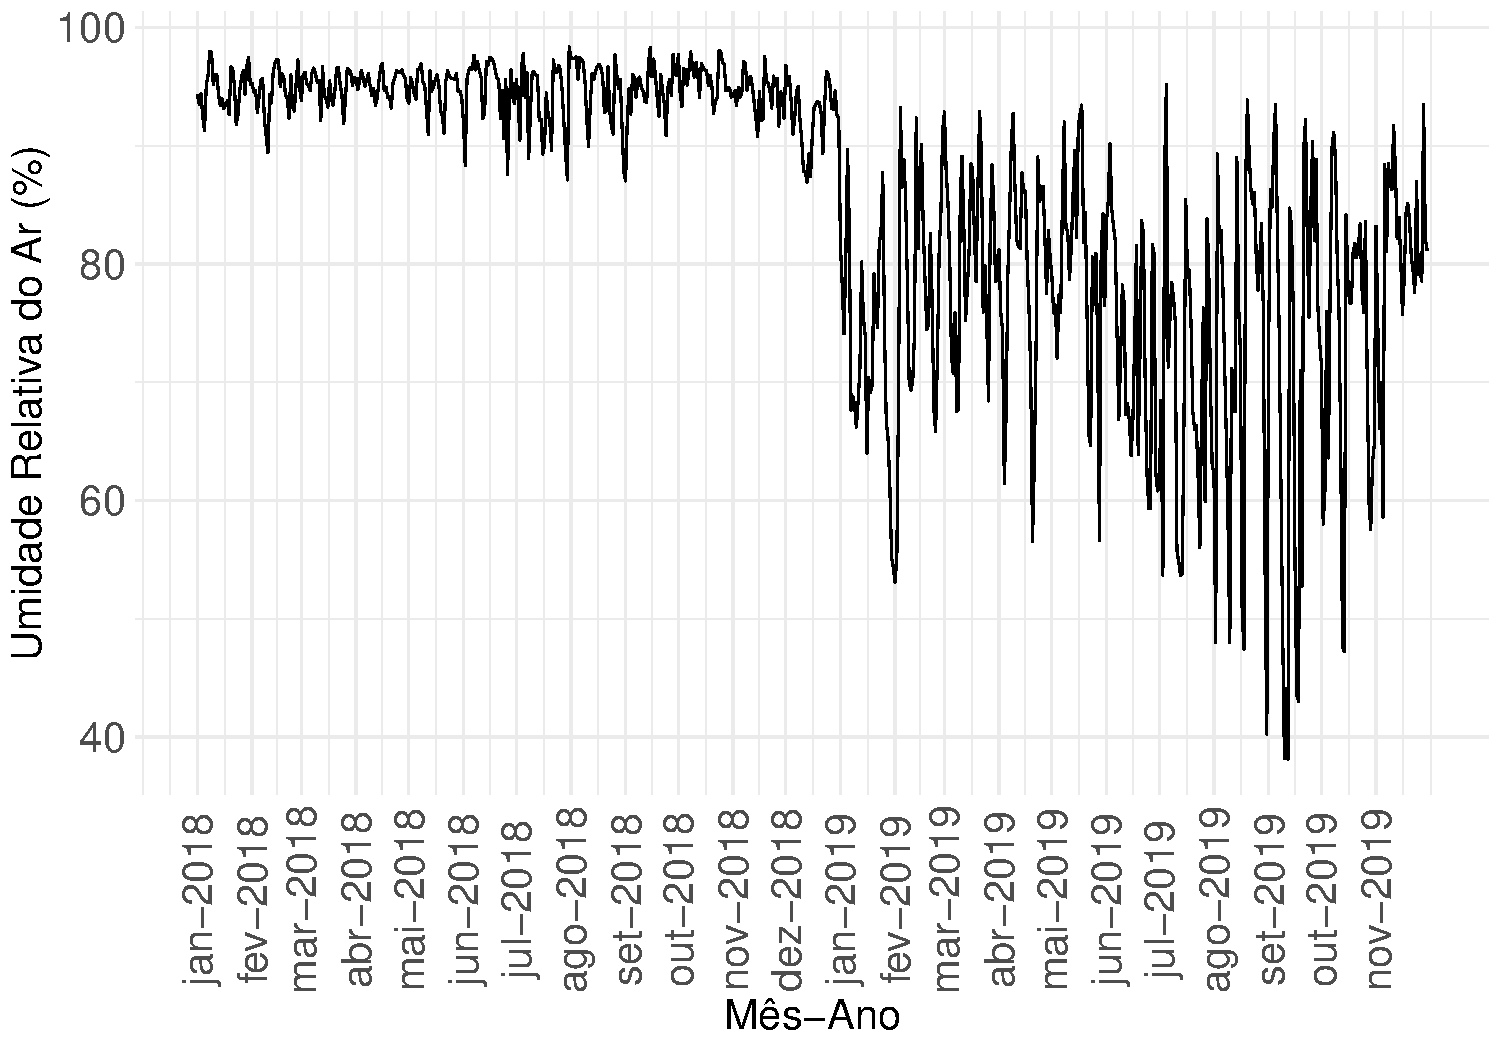
\includegraphics[width=1\textwidth,height=\textheight]{apresentacao_files/figure-beamer/unnamed-chunk-9-1.pdf}
\end{frame}

\begin{frame}{Análise Descritiva}
\phantomsection\label{anuxe1lise-descritiva-2}
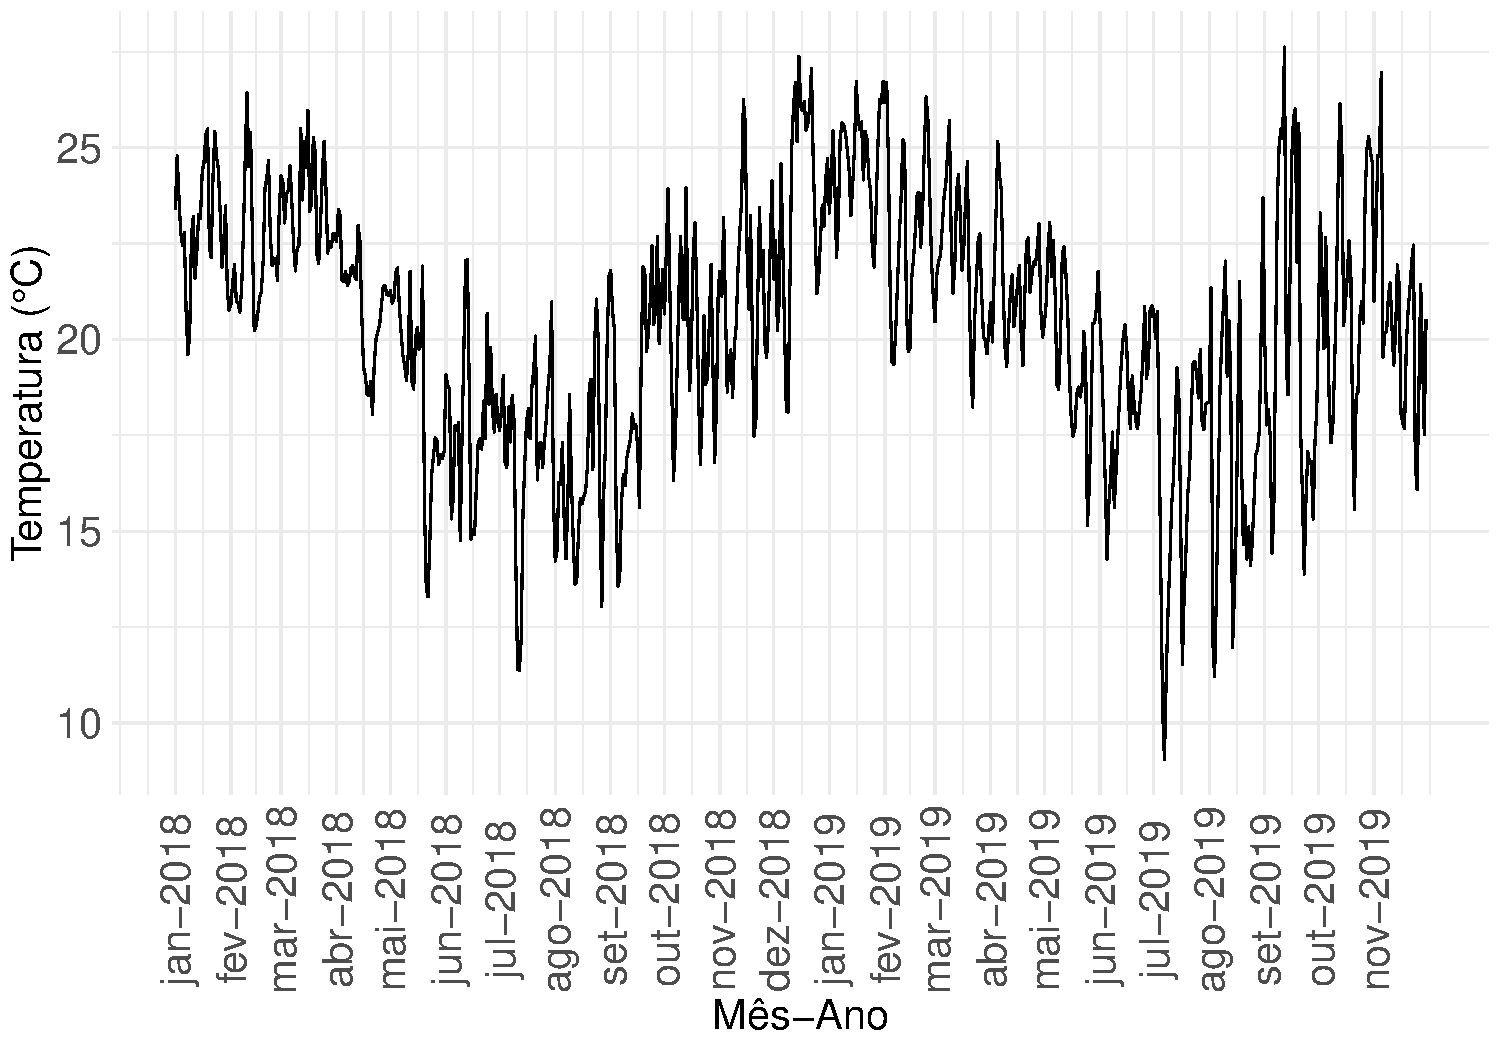
\includegraphics[width=1\textwidth,height=\textheight]{apresentacao_files/figure-beamer/unnamed-chunk-10-1.pdf}
\end{frame}

\begin{frame}{Análise Descritiva}
\phantomsection\label{anuxe1lise-descritiva-3}
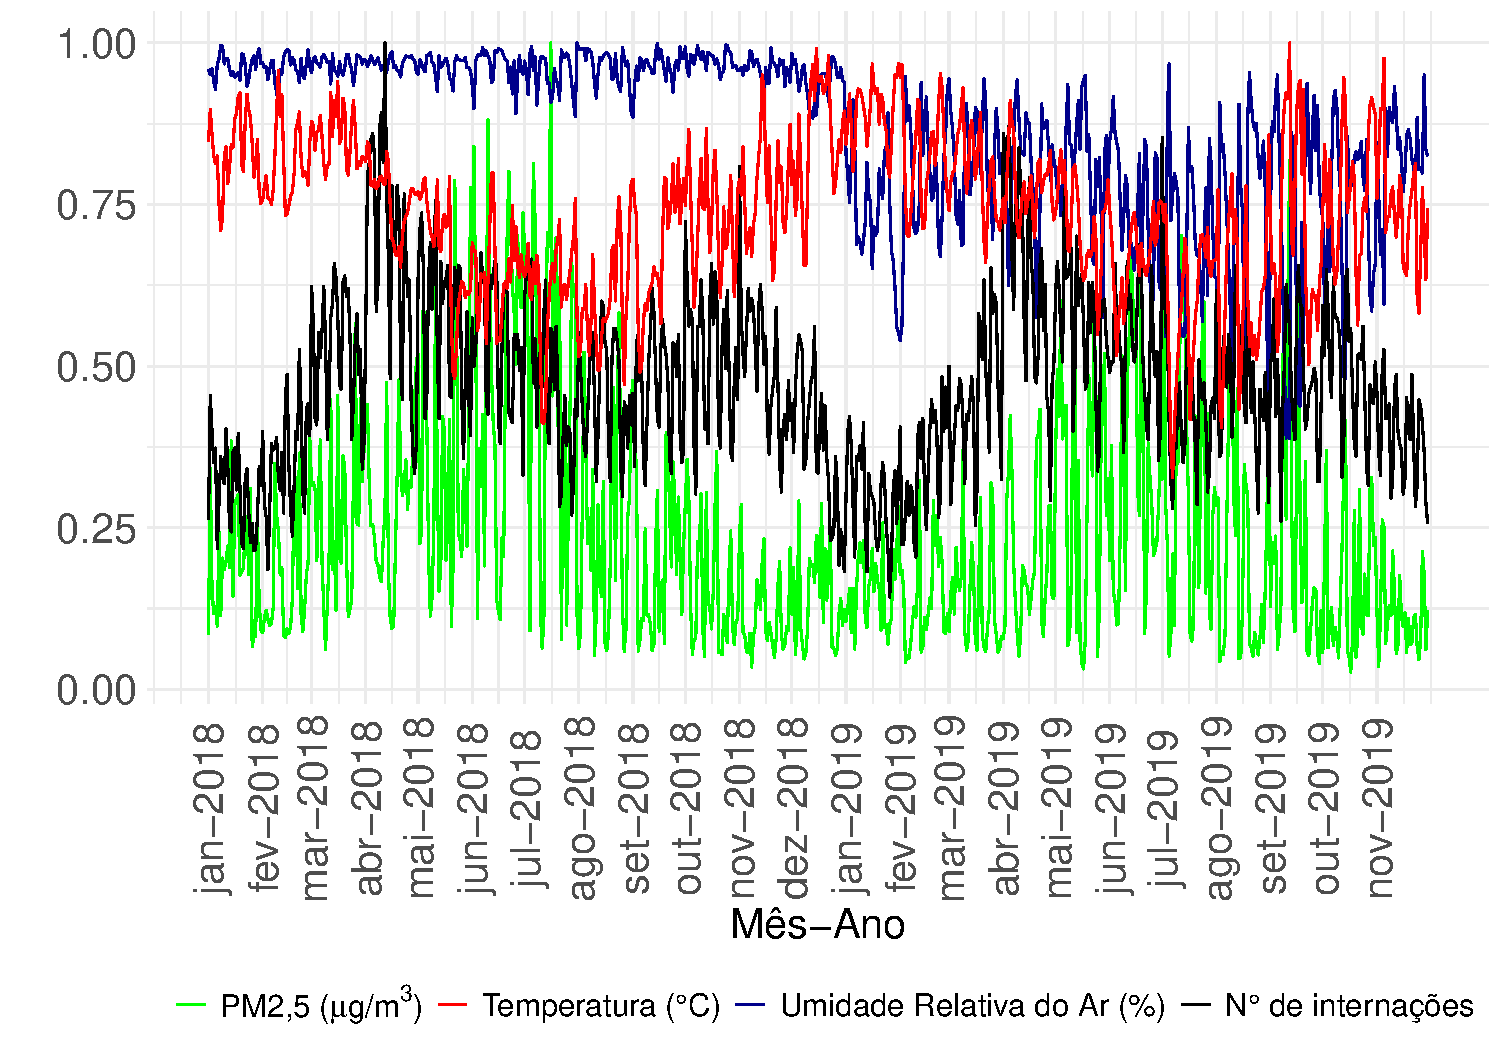
\includegraphics[width=1\textwidth,height=\textheight]{apresentacao_files/figure-beamer/unnamed-chunk-11-1.pdf}
\end{frame}

\section{Resultados}\label{resultados-1}

\begin{frame}{Resultados}
\phantomsection\label{resultados-2}
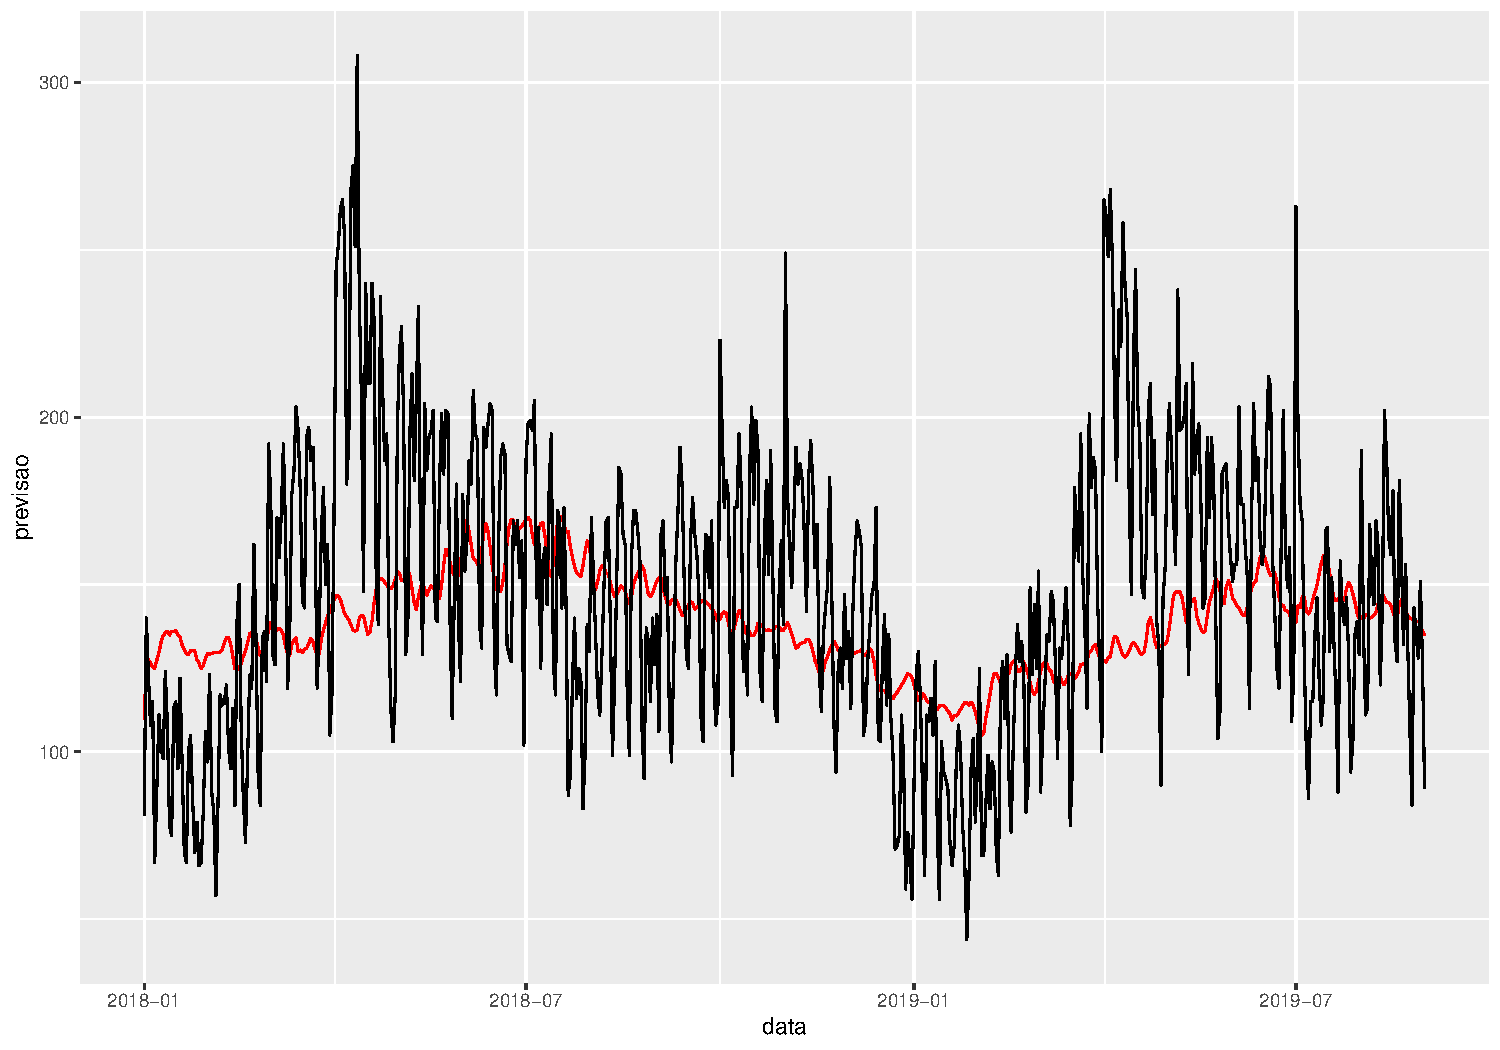
\includegraphics[width=1\textwidth,height=\textheight]{apresentacao_files/figure-beamer/unnamed-chunk-12-1.pdf}
\end{frame}

\begin{frame}{Resultados}
\phantomsection\label{resultados-3}
\begin{longtable}[]{@{}llll@{}}
\toprule\noalign{}
Modelo & RMSE & Rsquared & MAE \\
\midrule\noalign{}
\endhead
Modelo Completo (lag = 3) & 42,1282 & 0,0933 & 33,7120 \\
Modelo s/ Umidade (lag = 3) & 42,1282 & 0,0933 & 33,7120 \\
Modelo s/Umidade (lag = 7) & 55,9767 & 0,0079 & 42,6284 \\
Modelo s/Umidade (lag = 1) & 45,8886 & 0,0805 & 38,0505 \\
\bottomrule\noalign{}
\end{longtable}

\textsubscript{Tabela:~Métricas~do~modelo~da~base~treino~(Jan~de~2018~a~Ago~de~2019).}
\end{frame}

\begin{frame}{Resultados}
\phantomsection\label{resultados-4}
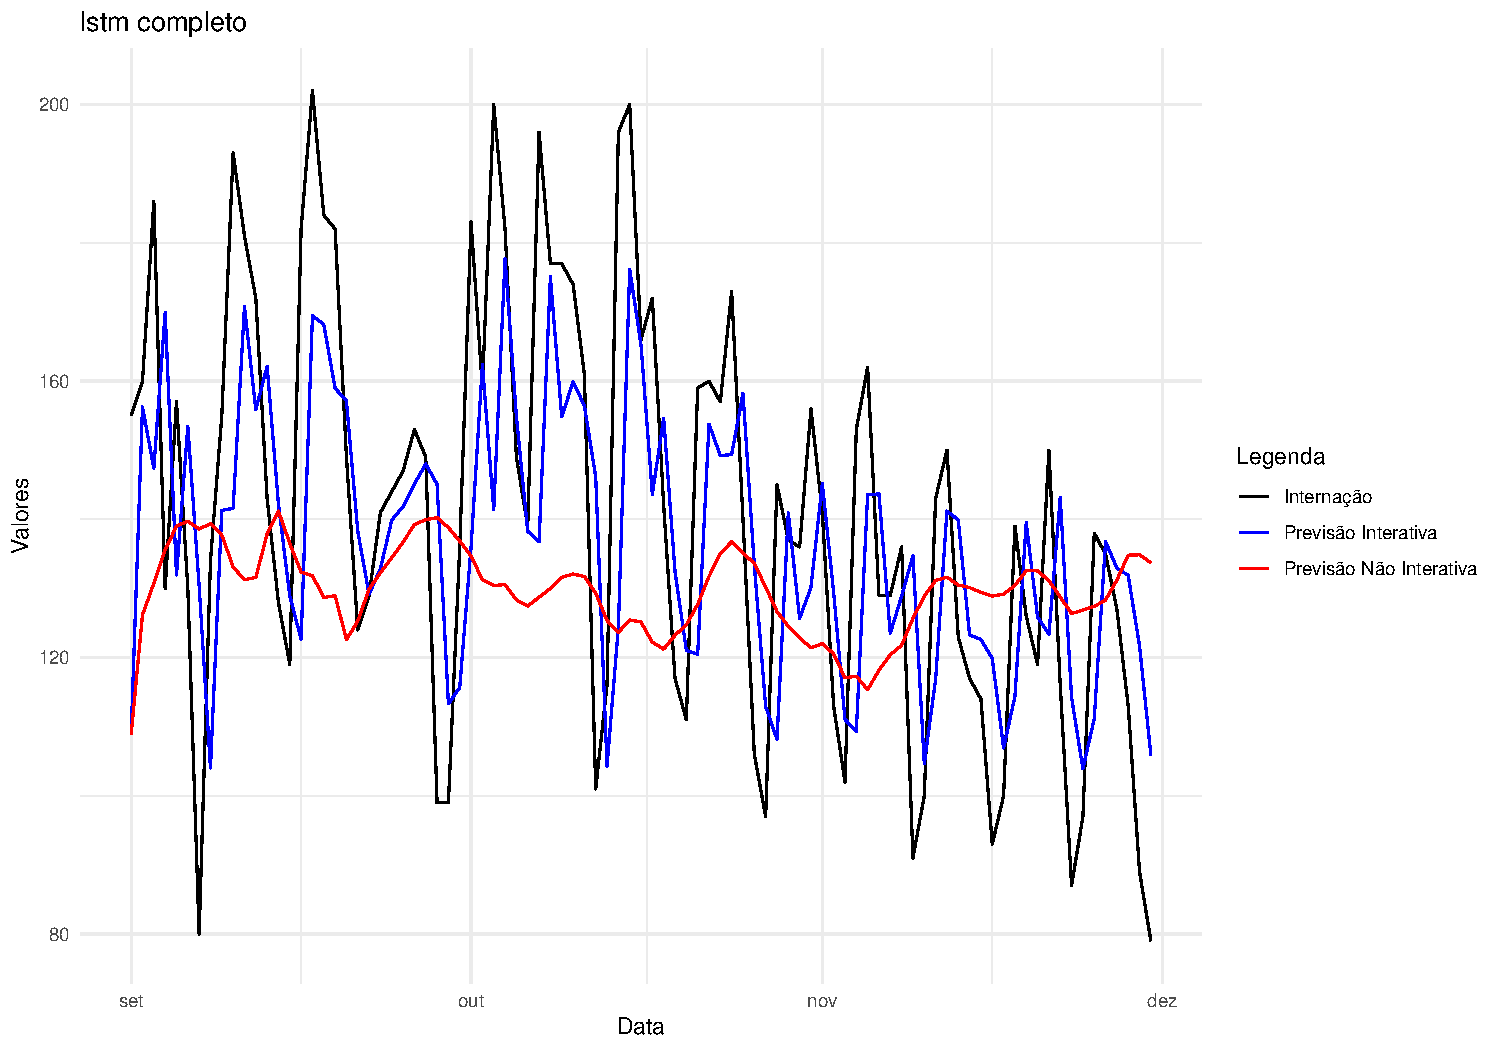
\includegraphics[width=1\textwidth,height=\textheight]{apresentacao_files/figure-beamer/unnamed-chunk-13-1.pdf}
\end{frame}

\begin{frame}{Resultados}
\phantomsection\label{resultados-5}
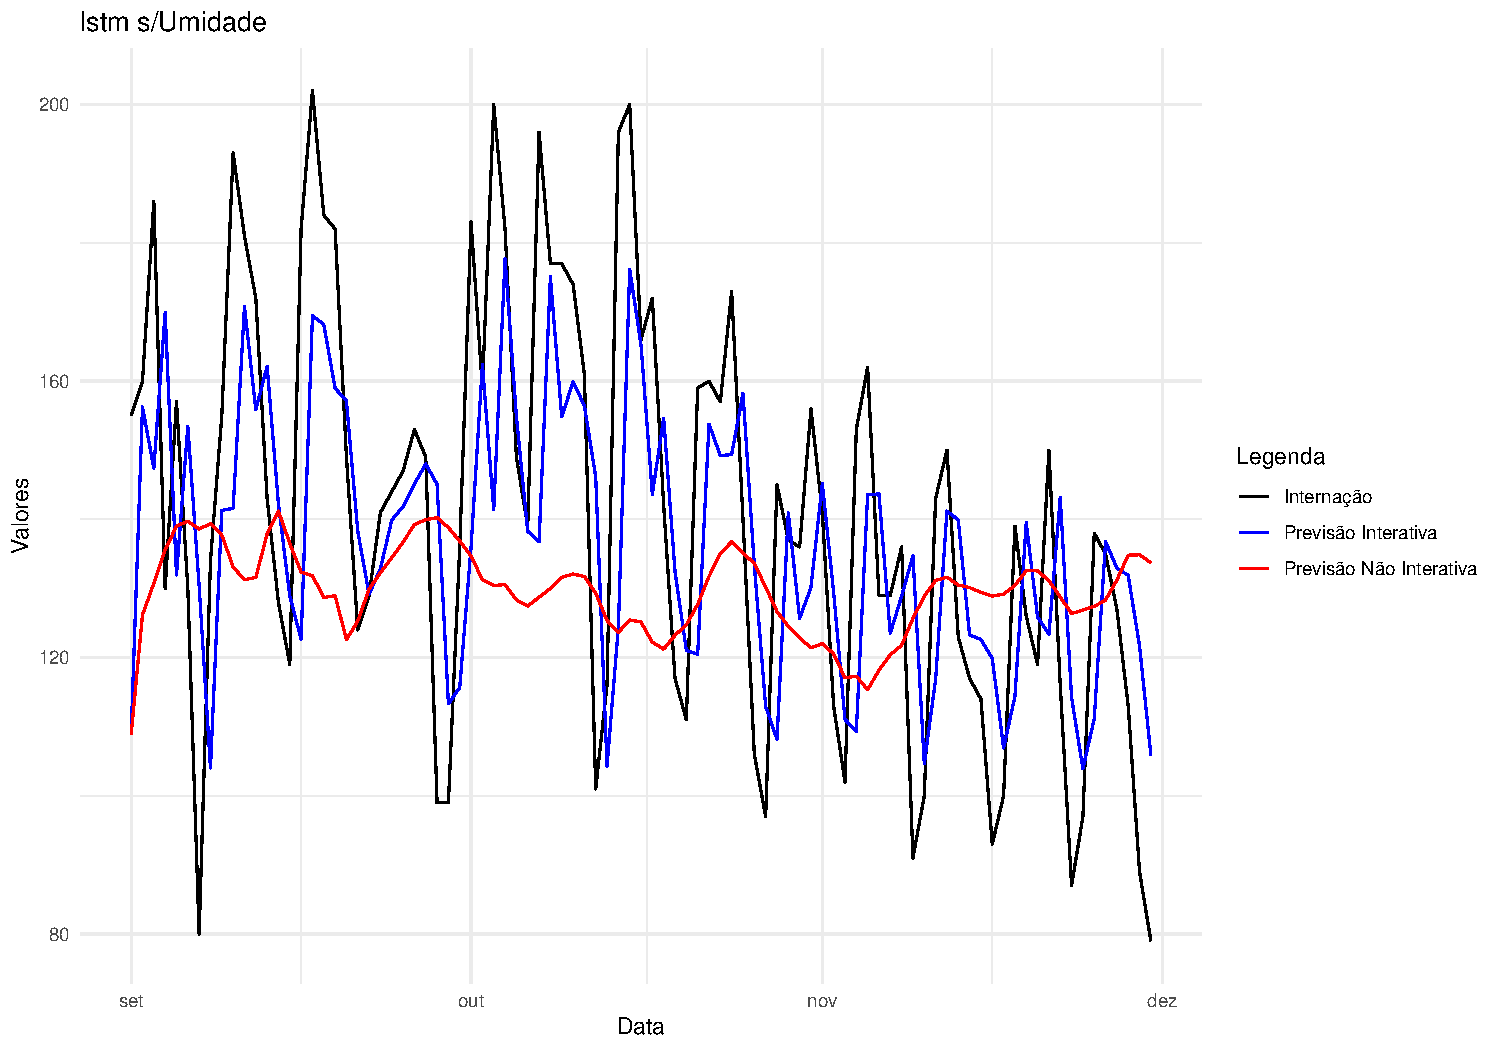
\includegraphics[width=1\textwidth,height=\textheight]{apresentacao_files/figure-beamer/unnamed-chunk-14-1.pdf}
\end{frame}

\begin{frame}{Resultados}
\phantomsection\label{resultados-6}
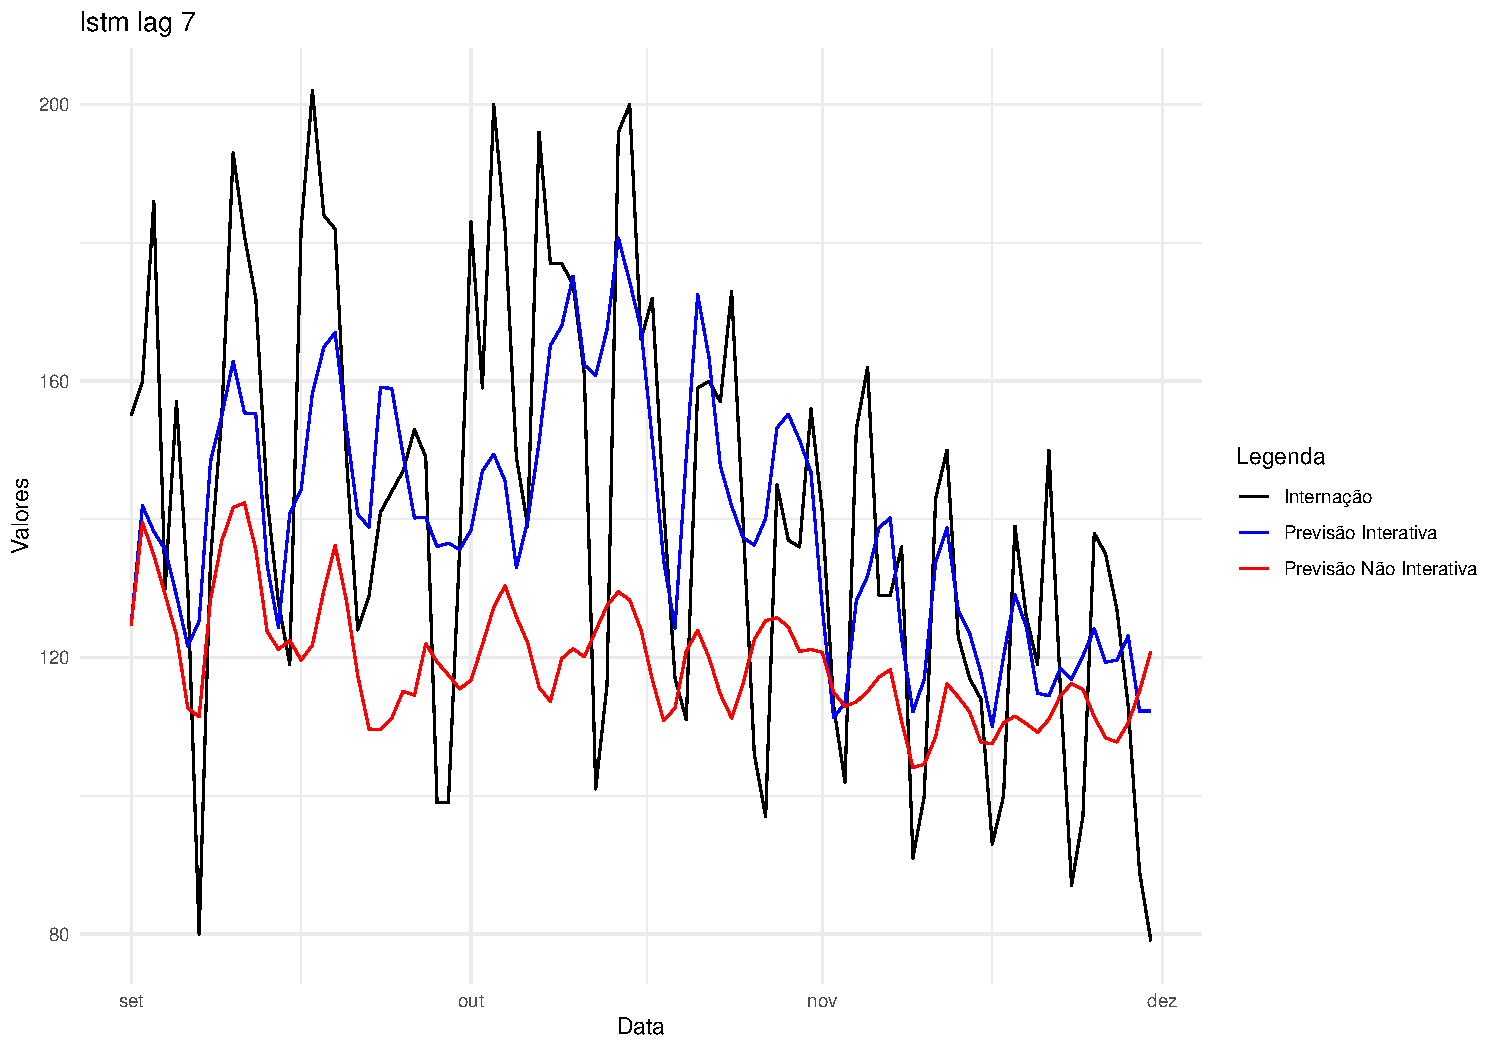
\includegraphics[width=1\textwidth,height=\textheight]{apresentacao_files/figure-beamer/unnamed-chunk-15-1.pdf}
\end{frame}

\begin{frame}{Resultados}
\phantomsection\label{resultados-7}
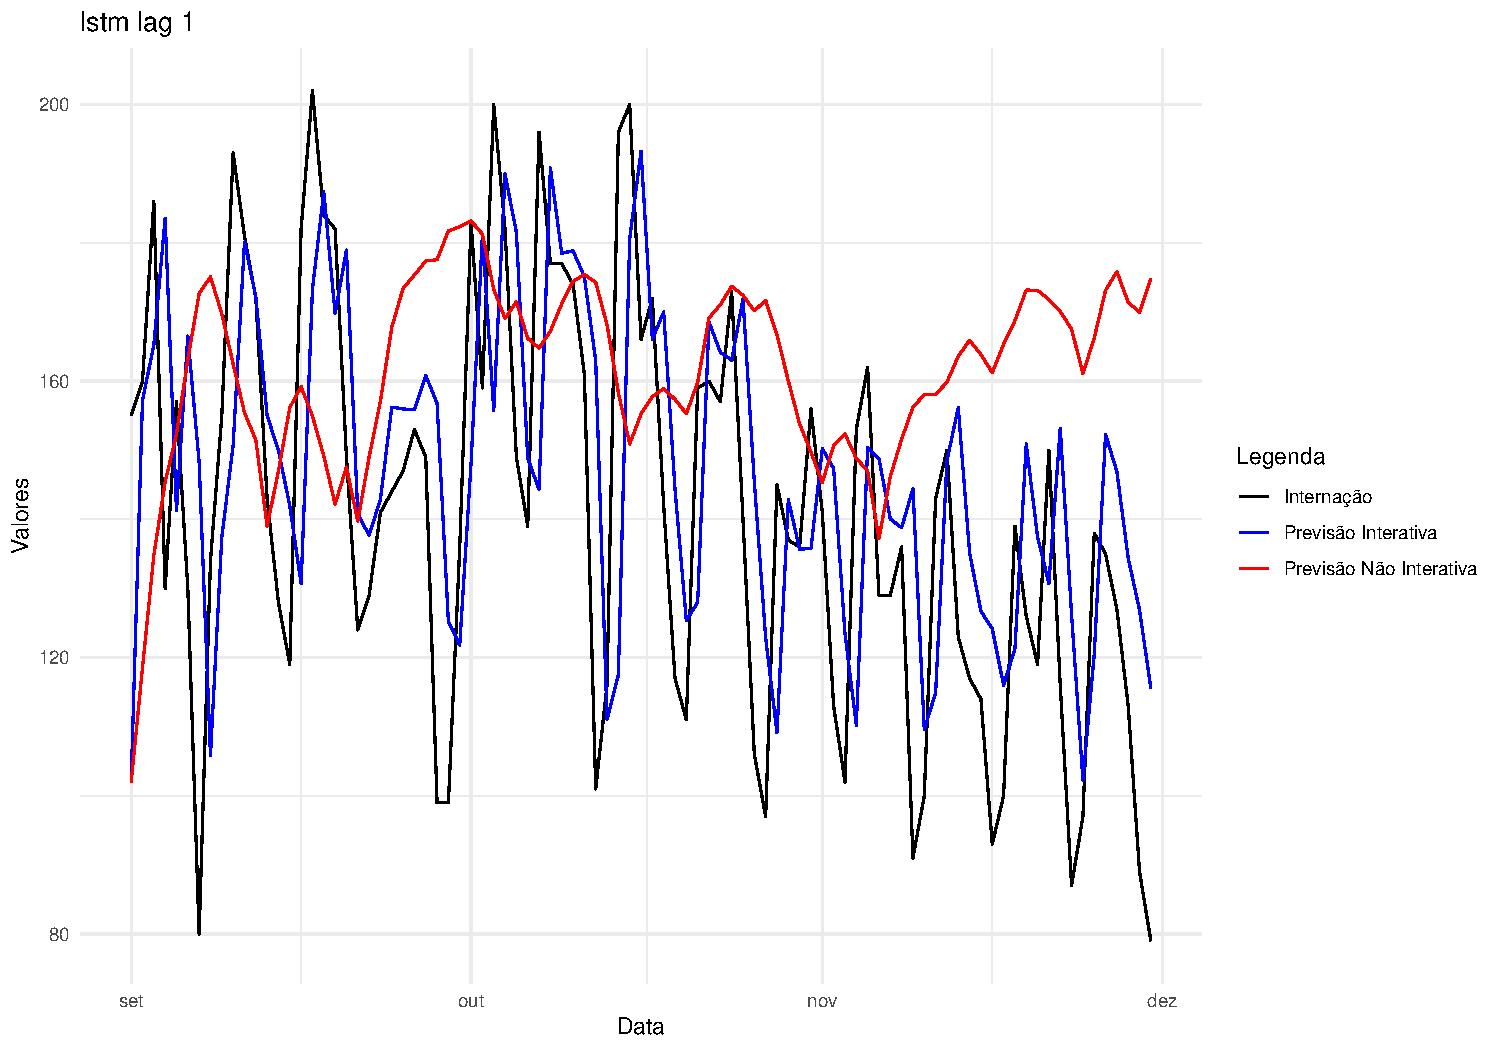
\includegraphics[width=1\textwidth,height=\textheight]{apresentacao_files/figure-beamer/unnamed-chunk-16-1.pdf}
\end{frame}

\begin{frame}{Resultados}
\phantomsection\label{resultados-8}
\begin{longtable}[]{@{}llll@{}}
\toprule\noalign{}
Modelo & RMSE & Rsquared & MAE \\
\midrule\noalign{}
\endhead
Modelo Completo (lag = 3) & 25,6221 & 0,3163 & 20,0272 \\
Modelo s/ Umidade (lag = 3) & 25,6221 & 0,3163 & 20,0272 \\
Modelo s/Umidade (lag = 7) & 23,0609 & 0,4388 & 18,2464 \\
Modelo s/Umidade (lag = 1) & 28,2284 & 0,2441 & 22,7946 \\
\bottomrule\noalign{}
\end{longtable}

\textsubscript{Tabela:~Métricas~do~modelo~da~base~teste~(Set-Out-Nov~de~2019).}
\end{frame}

\begin{frame}{Conclusão}
\phantomsection\label{conclusuxe3o}
\begin{itemize}
\tightlist
\item
  A umidade não alterou significativamente as estimativas e previsão do
  modelo, talvez devido ao seu comportamento problemático em 2018;
\item
  Mesmo com diversos modelos testados, foi difícil realizar uma boa
  previsão;
\item
  Pode-se, no futuro, evoluir a complexidade do modelo para obter-se
  melhores estimativas e explorar mais os \(lags\) para o modelo.
\end{itemize}
\end{frame}

\begin{frame}{Referências}
\phantomsection\label{referuxeancias}
\phantomsection\label{refs}
\begin{CSLReferences}{1}{0}
\bibitem[\citeproctext]{ref-A_Abdo_2012}
Arbex, Marcos Abdo. 2012. {``A Poluição Do Ar e o Sistema
Respiratório.''} \emph{Jornal Brasileiro de Pneumologia} 38 (5):
643--55. \url{https://doi.org/10.1590/s1806-37132012000500015}.

\bibitem[\citeproctext]{ref-L_Bengio_1994}
Bengio, Y. 1994. {``Learning Long-Term Dependencies with Gradient
Descent Is Difficult.''} \emph{IEEE Transactions on Neural Networks} 5
(2): 157--66. \url{https://doi.org/10.1109/72.279181}.

\end{CSLReferences}
\end{frame}



\end{document}
